% Options for packages loaded elsewhere
\PassOptionsToPackage{unicode}{hyperref}
\PassOptionsToPackage{hyphens}{url}
%
\documentclass[
]{article}
\usepackage{lmodern}
\usepackage{amsmath}
\usepackage{ifxetex,ifluatex}
\ifnum 0\ifxetex 1\fi\ifluatex 1\fi=0 % if pdftex
  \usepackage[T1]{fontenc}
  \usepackage[utf8]{inputenc}
  \usepackage{textcomp} % provide euro and other symbols
  \usepackage{amssymb}
\else % if luatex or xetex
  \usepackage{unicode-math}
  \defaultfontfeatures{Scale=MatchLowercase}
  \defaultfontfeatures[\rmfamily]{Ligatures=TeX,Scale=1}
\fi
% Use upquote if available, for straight quotes in verbatim environments
\IfFileExists{upquote.sty}{\usepackage{upquote}}{}
\IfFileExists{microtype.sty}{% use microtype if available
  \usepackage[]{microtype}
  \UseMicrotypeSet[protrusion]{basicmath} % disable protrusion for tt fonts
}{}
\makeatletter
\@ifundefined{KOMAClassName}{% if non-KOMA class
  \IfFileExists{parskip.sty}{%
    \usepackage{parskip}
  }{% else
    \setlength{\parindent}{0pt}
    \setlength{\parskip}{6pt plus 2pt minus 1pt}}
}{% if KOMA class
  \KOMAoptions{parskip=half}}
\makeatother
\usepackage{xcolor}
\IfFileExists{xurl.sty}{\usepackage{xurl}}{} % add URL line breaks if available
\IfFileExists{bookmark.sty}{\usepackage{bookmark}}{\usepackage{hyperref}}
\hypersetup{
  pdftitle={Options dans le cadre Black-Scholes},
  hidelinks,
  pdfcreator={LaTeX via pandoc}}
\urlstyle{same} % disable monospaced font for URLs
\usepackage[margin=1in]{geometry}
\usepackage{color}
\usepackage{fancyvrb}
\newcommand{\VerbBar}{|}
\newcommand{\VERB}{\Verb[commandchars=\\\{\}]}
\DefineVerbatimEnvironment{Highlighting}{Verbatim}{commandchars=\\\{\}}
% Add ',fontsize=\small' for more characters per line
\usepackage{framed}
\definecolor{shadecolor}{RGB}{248,248,248}
\newenvironment{Shaded}{\begin{snugshade}}{\end{snugshade}}
\newcommand{\AlertTok}[1]{\textcolor[rgb]{0.94,0.16,0.16}{#1}}
\newcommand{\AnnotationTok}[1]{\textcolor[rgb]{0.56,0.35,0.01}{\textbf{\textit{#1}}}}
\newcommand{\AttributeTok}[1]{\textcolor[rgb]{0.77,0.63,0.00}{#1}}
\newcommand{\BaseNTok}[1]{\textcolor[rgb]{0.00,0.00,0.81}{#1}}
\newcommand{\BuiltInTok}[1]{#1}
\newcommand{\CharTok}[1]{\textcolor[rgb]{0.31,0.60,0.02}{#1}}
\newcommand{\CommentTok}[1]{\textcolor[rgb]{0.56,0.35,0.01}{\textit{#1}}}
\newcommand{\CommentVarTok}[1]{\textcolor[rgb]{0.56,0.35,0.01}{\textbf{\textit{#1}}}}
\newcommand{\ConstantTok}[1]{\textcolor[rgb]{0.00,0.00,0.00}{#1}}
\newcommand{\ControlFlowTok}[1]{\textcolor[rgb]{0.13,0.29,0.53}{\textbf{#1}}}
\newcommand{\DataTypeTok}[1]{\textcolor[rgb]{0.13,0.29,0.53}{#1}}
\newcommand{\DecValTok}[1]{\textcolor[rgb]{0.00,0.00,0.81}{#1}}
\newcommand{\DocumentationTok}[1]{\textcolor[rgb]{0.56,0.35,0.01}{\textbf{\textit{#1}}}}
\newcommand{\ErrorTok}[1]{\textcolor[rgb]{0.64,0.00,0.00}{\textbf{#1}}}
\newcommand{\ExtensionTok}[1]{#1}
\newcommand{\FloatTok}[1]{\textcolor[rgb]{0.00,0.00,0.81}{#1}}
\newcommand{\FunctionTok}[1]{\textcolor[rgb]{0.00,0.00,0.00}{#1}}
\newcommand{\ImportTok}[1]{#1}
\newcommand{\InformationTok}[1]{\textcolor[rgb]{0.56,0.35,0.01}{\textbf{\textit{#1}}}}
\newcommand{\KeywordTok}[1]{\textcolor[rgb]{0.13,0.29,0.53}{\textbf{#1}}}
\newcommand{\NormalTok}[1]{#1}
\newcommand{\OperatorTok}[1]{\textcolor[rgb]{0.81,0.36,0.00}{\textbf{#1}}}
\newcommand{\OtherTok}[1]{\textcolor[rgb]{0.56,0.35,0.01}{#1}}
\newcommand{\PreprocessorTok}[1]{\textcolor[rgb]{0.56,0.35,0.01}{\textit{#1}}}
\newcommand{\RegionMarkerTok}[1]{#1}
\newcommand{\SpecialCharTok}[1]{\textcolor[rgb]{0.00,0.00,0.00}{#1}}
\newcommand{\SpecialStringTok}[1]{\textcolor[rgb]{0.31,0.60,0.02}{#1}}
\newcommand{\StringTok}[1]{\textcolor[rgb]{0.31,0.60,0.02}{#1}}
\newcommand{\VariableTok}[1]{\textcolor[rgb]{0.00,0.00,0.00}{#1}}
\newcommand{\VerbatimStringTok}[1]{\textcolor[rgb]{0.31,0.60,0.02}{#1}}
\newcommand{\WarningTok}[1]{\textcolor[rgb]{0.56,0.35,0.01}{\textbf{\textit{#1}}}}
\usepackage{graphicx}
\makeatletter
\def\maxwidth{\ifdim\Gin@nat@width>\linewidth\linewidth\else\Gin@nat@width\fi}
\def\maxheight{\ifdim\Gin@nat@height>\textheight\textheight\else\Gin@nat@height\fi}
\makeatother
% Scale images if necessary, so that they will not overflow the page
% margins by default, and it is still possible to overwrite the defaults
% using explicit options in \includegraphics[width, height, ...]{}
\setkeys{Gin}{width=\maxwidth,height=\maxheight,keepaspectratio}
% Set default figure placement to htbp
\makeatletter
\def\fps@figure{htbp}
\makeatother
\setlength{\emergencystretch}{3em} % prevent overfull lines
\providecommand{\tightlist}{%
  \setlength{\itemsep}{0pt}\setlength{\parskip}{0pt}}
\setcounter{secnumdepth}{-\maxdimen} % remove section numbering
\usepackage[utf8]{inputenc}
\usepackage{amsmath}
\usepackage{amsfonts}
\usepackage{amssymb}
\ifluatex
  \usepackage{selnolig}  % disable illegal ligatures
\fi

\title{Options dans le cadre Black-Scholes}
\usepackage{etoolbox}
\makeatletter
\providecommand{\subtitle}[1]{% add subtitle to \maketitle
  \apptocmd{\@title}{\par {\large #1 \par}}{}{}
}
\makeatother
\subtitle{TP-2: Pricing Vanna-Volga}
\author{}
\date{\vspace{-2.5em}Version: 22 mar 2022}

\begin{document}
\maketitle

The purpose of this problem set is to explore the Vanna-Volga pricing
model. In this problem set, you will use the following functions:

GBSPrice: Price of a vanilla option: \[
P = f(\text{PutCall}, S, K, T, r, b, \sigma)
\]

where:

\begin{description}
\item[PutCall] 'c' for a call, 'p' for a put
\item[$b$] cost of carry: ridk free rate $r$ less dividend yield $d$
\item[$r$] risk-free rate
\end{description}

\begin{Shaded}
\begin{Highlighting}[]
\NormalTok{GBSPrice }\OtherTok{\textless{}{-}} \ControlFlowTok{function}\NormalTok{(PutCall, S, K, T, r, b, sigma) \{}
\NormalTok{  d1 }\OtherTok{\textless{}{-}}\NormalTok{ (}\FunctionTok{log}\NormalTok{(S}\SpecialCharTok{/}\NormalTok{K) }\SpecialCharTok{+}\NormalTok{ (b}\SpecialCharTok{+}\NormalTok{sigma}\SpecialCharTok{\^{}}\DecValTok{2}\SpecialCharTok{/}\DecValTok{2}\NormalTok{)}\SpecialCharTok{*}\NormalTok{T)}\SpecialCharTok{/}\NormalTok{(sigma}\SpecialCharTok{*}\FunctionTok{sqrt}\NormalTok{(T))}
\NormalTok{  d2 }\OtherTok{\textless{}{-}}\NormalTok{ d1 }\SpecialCharTok{{-}}\NormalTok{ sigma}\SpecialCharTok{*}\FunctionTok{sqrt}\NormalTok{(T)}

  \ControlFlowTok{if}\NormalTok{(PutCall }\SpecialCharTok{==} \StringTok{\textquotesingle{}c\textquotesingle{}}\NormalTok{)  }
\NormalTok{    px }\OtherTok{\textless{}{-}}\NormalTok{ S}\SpecialCharTok{*}\FunctionTok{exp}\NormalTok{((b}\SpecialCharTok{{-}}\NormalTok{r)}\SpecialCharTok{*}\NormalTok{T)}\SpecialCharTok{*}\FunctionTok{pnorm}\NormalTok{(d1) }\SpecialCharTok{{-}}\NormalTok{ K}\SpecialCharTok{*}\FunctionTok{exp}\NormalTok{(}\SpecialCharTok{{-}}\NormalTok{r}\SpecialCharTok{*}\NormalTok{T)}\SpecialCharTok{*}\FunctionTok{pnorm}\NormalTok{(d2)}
  \ControlFlowTok{else}
\NormalTok{    px }\OtherTok{\textless{}{-}}\NormalTok{ K}\SpecialCharTok{*}\FunctionTok{exp}\NormalTok{(}\SpecialCharTok{{-}}\NormalTok{r}\SpecialCharTok{*}\NormalTok{T)}\SpecialCharTok{*}\FunctionTok{pnorm}\NormalTok{(}\SpecialCharTok{{-}}\NormalTok{d2) }\SpecialCharTok{{-}}\NormalTok{ S}\SpecialCharTok{*}\FunctionTok{exp}\NormalTok{((b}\SpecialCharTok{{-}}\NormalTok{r)}\SpecialCharTok{*}\NormalTok{T)}\SpecialCharTok{*}\FunctionTok{pnorm}\NormalTok{(}\SpecialCharTok{{-}}\NormalTok{d1)}

\NormalTok{px}
\NormalTok{\}}
\end{Highlighting}
\end{Shaded}

GBSVega: Vega (\(\frac{\partial P}{\partial \sigma}\)) of a Vanilla
option:

\begin{Shaded}
\begin{Highlighting}[]
\NormalTok{GBSVega }\OtherTok{\textless{}{-}} \ControlFlowTok{function}\NormalTok{(PutCall, S, K, T, r, b, sigma) \{}
\NormalTok{  d1 }\OtherTok{\textless{}{-}}\NormalTok{ (}\FunctionTok{log}\NormalTok{(S}\SpecialCharTok{/}\NormalTok{K) }\SpecialCharTok{+}\NormalTok{ (b}\SpecialCharTok{+}\NormalTok{sigma}\SpecialCharTok{\^{}}\DecValTok{2}\SpecialCharTok{/}\DecValTok{2}\NormalTok{)}\SpecialCharTok{*}\NormalTok{T)}\SpecialCharTok{/}\NormalTok{(sigma}\SpecialCharTok{*}\FunctionTok{sqrt}\NormalTok{(T))}
\NormalTok{  S}\SpecialCharTok{*}\FunctionTok{exp}\NormalTok{((b}\SpecialCharTok{{-}}\NormalTok{r)}\SpecialCharTok{*}\NormalTok{T) }\SpecialCharTok{*} \FunctionTok{dnorm}\NormalTok{(d1)}
\NormalTok{\}}
\end{Highlighting}
\end{Shaded}

\hypertarget{volatility-interpolation}{%
\section{Volatility Interpolation}\label{volatility-interpolation}}

Given the implied volatility at three strikes, we will use the
Vanna-Volga pricing method to interpolate the volatility curve. Assume
\(r=0, b=0, T=1, \mbox{Spot} = 100\).

\begin{Shaded}
\begin{Highlighting}[]
\CommentTok{\# Benchmark data: (strike, volatility)}
\NormalTok{VolData }\OtherTok{\textless{}{-}} \FunctionTok{list}\NormalTok{(}\FunctionTok{c}\NormalTok{(}\DecValTok{80}\NormalTok{, .}\DecValTok{32}\NormalTok{), }\FunctionTok{c}\NormalTok{(}\DecValTok{100}\NormalTok{, .}\DecValTok{30}\NormalTok{), }\FunctionTok{c}\NormalTok{(}\DecValTok{120}\NormalTok{, .}\DecValTok{315}\NormalTok{))}
\end{Highlighting}
\end{Shaded}

Let's first define an array of pricing functions for the benchmark
instruments:

\begin{Shaded}
\begin{Highlighting}[]
\NormalTok{C1 }\OtherTok{\textless{}{-}} \ControlFlowTok{function}\NormalTok{(}\AttributeTok{vol=}\NormalTok{sigma, }\AttributeTok{spot=}\NormalTok{Spot) }\FunctionTok{GBSPrice}\NormalTok{(}\AttributeTok{PutCall=}\StringTok{\textquotesingle{}c\textquotesingle{}}\NormalTok{, }\AttributeTok{S=}\NormalTok{spot, }\AttributeTok{K=}\NormalTok{VolData[[}\DecValTok{1}\NormalTok{]][}\DecValTok{1}\NormalTok{], }\AttributeTok{T=}\NormalTok{T, }\AttributeTok{r=}\NormalTok{r, }\AttributeTok{b=}\NormalTok{b, }\AttributeTok{sigma=}\NormalTok{vol)}

\NormalTok{C2 }\OtherTok{\textless{}{-}} \ControlFlowTok{function}\NormalTok{(}\AttributeTok{vol=}\NormalTok{sigma, }\AttributeTok{spot=}\NormalTok{Spot) }\FunctionTok{GBSPrice}\NormalTok{(}\AttributeTok{PutCall=}\StringTok{\textquotesingle{}c\textquotesingle{}}\NormalTok{, }\AttributeTok{S=}\NormalTok{spot, }\AttributeTok{K=}\NormalTok{VolData[[}\DecValTok{2}\NormalTok{]][}\DecValTok{1}\NormalTok{], }\AttributeTok{T=}\NormalTok{T, }\AttributeTok{r=}\NormalTok{r, }\AttributeTok{b=}\NormalTok{b, }\AttributeTok{sigma=}\NormalTok{vol)}

\NormalTok{C3 }\OtherTok{\textless{}{-}} \ControlFlowTok{function}\NormalTok{(}\AttributeTok{vol=}\NormalTok{sigma, }\AttributeTok{spot=}\NormalTok{Spot) }\FunctionTok{GBSPrice}\NormalTok{(}\AttributeTok{PutCall=}\StringTok{\textquotesingle{}c\textquotesingle{}}\NormalTok{, }\AttributeTok{S=}\NormalTok{spot, }\AttributeTok{K=}\NormalTok{VolData[[}\DecValTok{3}\NormalTok{]][}\DecValTok{1}\NormalTok{], }\AttributeTok{T=}\NormalTok{T, }\AttributeTok{r=}\NormalTok{r, }\AttributeTok{b=}\NormalTok{b, }\AttributeTok{sigma=}\NormalTok{vol)}

\NormalTok{C }\OtherTok{\textless{}{-}} \FunctionTok{c}\NormalTok{(C1, C2, C3)}
\end{Highlighting}
\end{Shaded}

\begin{enumerate}
\def\labelenumi{\arabic{enumi}.}
\tightlist
\item
  Write a utility functions to compute the risk indicators, all by
  finite difference:
\end{enumerate}

\begin{Shaded}
\begin{Highlighting}[]
\NormalTok{Vega }\OtherTok{\textless{}{-}} \ControlFlowTok{function}\NormalTok{(f, vol, }\AttributeTok{spot=}\NormalTok{Spot) \{}
\NormalTok{  d\_vol }\OtherTok{\textless{}{-}} \FloatTok{10e{-}5}
  \FunctionTok{return}\NormalTok{( (}\FunctionTok{f}\NormalTok{(vol}\SpecialCharTok{+}\NormalTok{d\_vol}\SpecialCharTok{*}\NormalTok{vol, Spot)}\SpecialCharTok{{-}}\FunctionTok{f}\NormalTok{(vol}\SpecialCharTok{{-}}\NormalTok{d\_vol}\SpecialCharTok{*}\NormalTok{vol, Spot))}\SpecialCharTok{/}\NormalTok{(}\DecValTok{2}\SpecialCharTok{*}\NormalTok{d\_vol) )}
\NormalTok{\}}

\NormalTok{Vanna }\OtherTok{\textless{}{-}} \ControlFlowTok{function}\NormalTok{(f, vol, }\AttributeTok{spot=}\NormalTok{Spot) \{}
\NormalTok{  d\_vol }\OtherTok{\textless{}{-}} \FloatTok{10e{-}5}
\NormalTok{  d\_spot }\OtherTok{\textless{}{-}} \FloatTok{10e{-}5}
  \FunctionTok{return}\NormalTok{( (}\FunctionTok{f}\NormalTok{(vol}\SpecialCharTok{+}\NormalTok{d\_vol}\SpecialCharTok{*}\NormalTok{vol, Spot}\SpecialCharTok{+}\NormalTok{d\_spot}\SpecialCharTok{*}\NormalTok{Spot)}\SpecialCharTok{+}
           \FunctionTok{f}\NormalTok{(vol}\SpecialCharTok{{-}}\NormalTok{d\_vol}\SpecialCharTok{*}\NormalTok{vol, Spot}\SpecialCharTok{{-}}\NormalTok{d\_spot}\SpecialCharTok{*}\NormalTok{Spot)}\SpecialCharTok{{-}}
           \FunctionTok{f}\NormalTok{(vol}\SpecialCharTok{+}\NormalTok{d\_vol}\SpecialCharTok{*}\NormalTok{vol, Spot}\SpecialCharTok{{-}}\NormalTok{d\_spot}\SpecialCharTok{*}\NormalTok{Spot)}\SpecialCharTok{{-}}
           \FunctionTok{f}\NormalTok{(vol}\SpecialCharTok{{-}}\NormalTok{d\_vol}\SpecialCharTok{*}\NormalTok{vol, Spot}\SpecialCharTok{+}\NormalTok{d\_spot}\SpecialCharTok{*}\NormalTok{Spot))}\SpecialCharTok{/}\NormalTok{(}\DecValTok{4}\SpecialCharTok{*}\NormalTok{d\_vol}\SpecialCharTok{*}\NormalTok{d\_spot) )}
\NormalTok{\}}
  
\NormalTok{Volga }\OtherTok{\textless{}{-}} \ControlFlowTok{function}\NormalTok{(f, vol, }\AttributeTok{spot=}\NormalTok{Spot) \{}
\NormalTok{  d\_vol }\OtherTok{\textless{}{-}} \FloatTok{10e{-}5}
  \FunctionTok{return}\NormalTok{( (}\FunctionTok{f}\NormalTok{(vol}\SpecialCharTok{+}\NormalTok{d\_vol}\SpecialCharTok{*}\NormalTok{vol, Spot) }\SpecialCharTok{{-}} \DecValTok{2}\SpecialCharTok{*}\FunctionTok{f}\NormalTok{(vol, Spot) }\SpecialCharTok{+} \FunctionTok{f}\NormalTok{(vol}\SpecialCharTok{{-}}\NormalTok{d\_vol}\SpecialCharTok{*}\NormalTok{vol, Spot))}\SpecialCharTok{/}\NormalTok{d\_vol}\SpecialCharTok{**}\DecValTok{2}\NormalTok{ )}
\NormalTok{  \}}
\end{Highlighting}
\end{Shaded}

Then, the calculation of vega for the three benchmark options may be
performed by:

\begin{Shaded}
\begin{Highlighting}[]
\NormalTok{r}\OtherTok{\textless{}{-}}\DecValTok{0}
\NormalTok{b}\OtherTok{\textless{}{-}}\DecValTok{0}
\NormalTok{T}\OtherTok{\textless{}{-}}\DecValTok{1}
\NormalTok{Spot }\OtherTok{\textless{}{-}} \DecValTok{100}
\NormalTok{B.vega }\OtherTok{\textless{}{-}} \FunctionTok{sapply}\NormalTok{(}\DecValTok{1}\SpecialCharTok{:}\DecValTok{3}\NormalTok{, }\ControlFlowTok{function}\NormalTok{(i) }\FunctionTok{Vega}\NormalTok{(C[[i]], VolData[[i]][}\DecValTok{2}\NormalTok{]))}
\end{Highlighting}
\end{Shaded}

\begin{enumerate}
\def\labelenumi{\arabic{enumi}.}
\setcounter{enumi}{1}
\tightlist
\item
  Compute vectors of vega, vanna, volga for the three hedge instruments
\end{enumerate}

\begin{Shaded}
\begin{Highlighting}[]
\NormalTok{r}\OtherTok{\textless{}{-}}\DecValTok{0}
\NormalTok{b}\OtherTok{\textless{}{-}}\DecValTok{0}
\NormalTok{T}\OtherTok{\textless{}{-}}\DecValTok{1}
\NormalTok{Spot }\OtherTok{\textless{}{-}} \DecValTok{100}
\NormalTok{B.vega.benchmark }\OtherTok{\textless{}{-}} \FunctionTok{sapply}\NormalTok{(}\DecValTok{1}\SpecialCharTok{:}\DecValTok{3}\NormalTok{, }\ControlFlowTok{function}\NormalTok{(i) }\FunctionTok{Vega}\NormalTok{(C[[i]], VolData[[i]][}\DecValTok{2}\NormalTok{]))}
\NormalTok{B.vanna.benchmark }\OtherTok{\textless{}{-}} \FunctionTok{sapply}\NormalTok{(}\DecValTok{1}\SpecialCharTok{:}\DecValTok{3}\NormalTok{, }\ControlFlowTok{function}\NormalTok{(i) }\FunctionTok{Vanna}\NormalTok{(C[[i]], VolData[[i]][}\DecValTok{2}\NormalTok{]))}
\NormalTok{B.volga.benchmark }\OtherTok{\textless{}{-}} \FunctionTok{sapply}\NormalTok{(}\DecValTok{1}\SpecialCharTok{:}\DecValTok{3}\NormalTok{, }\ControlFlowTok{function}\NormalTok{(i) }\FunctionTok{Volga}\NormalTok{(C[[i]], VolData[[i]][}\DecValTok{2}\NormalTok{]))}
\FunctionTok{print}\NormalTok{(}\StringTok{"B.vega.benchmark for C1, C2 and C3"}\NormalTok{)}
\end{Highlighting}
\end{Shaded}

\begin{verbatim}
## [1] "B.vega.benchmark for C1, C2 and C3"
\end{verbatim}

\begin{Shaded}
\begin{Highlighting}[]
\NormalTok{B.vega.benchmark}
\end{Highlighting}
\end{Shaded}

\begin{verbatim}
## [1]  8.840076 11.834380 11.499491
\end{verbatim}

\begin{Shaded}
\begin{Highlighting}[]
\FunctionTok{print}\NormalTok{(}\StringTok{"B.vanna.benchmark for C1, C2 and C3"}\NormalTok{)}
\end{Highlighting}
\end{Shaded}

\begin{verbatim}
## [1] "B.vanna.benchmark for C1, C2 and C3"
\end{verbatim}

\begin{Shaded}
\begin{Highlighting}[]
\NormalTok{B.vanna.benchmark}
\end{Highlighting}
\end{Shaded}

\begin{verbatim}
## [1] -14.84369   5.91719  26.87955
\end{verbatim}

\begin{Shaded}
\begin{Highlighting}[]
\FunctionTok{print}\NormalTok{(}\StringTok{"B.volga.benchmark for C1, C2 and C3"}\NormalTok{)}
\end{Highlighting}
\end{Shaded}

\begin{verbatim}
## [1] "B.volga.benchmark for C1, C2 and C3"
\end{verbatim}

\begin{Shaded}
\begin{Highlighting}[]
\NormalTok{B.volga.benchmark}
\end{Highlighting}
\end{Shaded}

\begin{verbatim}
## [1]  4.0722703 -0.2662745  3.5671601
\end{verbatim}

\begin{enumerate}
\def\labelenumi{\arabic{enumi}.}
\setcounter{enumi}{2}
\item
  Choose a new strike for which we want to compute the implied
  volatility. Let's choose \(K=110\).
\item
  Compute the risk indicators for a call option struck at that strike.
\end{enumerate}

\begin{Shaded}
\begin{Highlighting}[]
\NormalTok{r}\OtherTok{\textless{}{-}}\DecValTok{0}
\NormalTok{b}\OtherTok{\textless{}{-}}\DecValTok{0}
\NormalTok{T}\OtherTok{\textless{}{-}}\DecValTok{1}
\NormalTok{Spot }\OtherTok{\textless{}{-}} \DecValTok{100}
\NormalTok{K }\OtherTok{\textless{}{-}} \DecValTok{110}


\NormalTok{VolData.ATM }\OtherTok{\textless{}{-}}\NormalTok{ VolData[[}\DecValTok{2}\NormalTok{]][}\DecValTok{2}\NormalTok{]}

\NormalTok{f }\OtherTok{\textless{}{-}} \ControlFlowTok{function}\NormalTok{(}\AttributeTok{vol=}\NormalTok{VolData.ATM, }\AttributeTok{spot=}\NormalTok{Spot)\{}
  \FunctionTok{GBSPrice}\NormalTok{(}\AttributeTok{PutCall=}\StringTok{\textquotesingle{}c\textquotesingle{}}\NormalTok{, }\AttributeTok{S=}\NormalTok{spot, }\AttributeTok{K=}\NormalTok{K, }\AttributeTok{T=}\NormalTok{T, }\AttributeTok{r=}\NormalTok{r, }\AttributeTok{b=}\NormalTok{b, }\AttributeTok{sigma=}\NormalTok{vol)}
\NormalTok{\}}
\NormalTok{B.vega }\OtherTok{\textless{}{-}} \FunctionTok{Vega}\NormalTok{(f, VolData.ATM, Spot)}
\NormalTok{B.vanna }\OtherTok{\textless{}{-}} \FunctionTok{Vanna}\NormalTok{(f, VolData.ATM, Spot)}
\NormalTok{B.volga }\OtherTok{\textless{}{-}} \FunctionTok{Volga}\NormalTok{(f, VolData.ATM, Spot)}
\FunctionTok{print}\NormalTok{(}\StringTok{"vega for K=110"}\NormalTok{)}
\end{Highlighting}
\end{Shaded}

\begin{verbatim}
## [1] "vega for K=110"
\end{verbatim}

\begin{Shaded}
\begin{Highlighting}[]
\NormalTok{B.vega}
\end{Highlighting}
\end{Shaded}

\begin{verbatim}
## [1] 11.80115
\end{verbatim}

\begin{Shaded}
\begin{Highlighting}[]
\FunctionTok{print}\NormalTok{(}\StringTok{"vanna for K=110"}\NormalTok{)}
\end{Highlighting}
\end{Shaded}

\begin{verbatim}
## [1] "vanna for K=110"
\end{verbatim}

\begin{Shaded}
\begin{Highlighting}[]
\NormalTok{B.vanna}
\end{Highlighting}
\end{Shaded}

\begin{verbatim}
## [1] 18.39802
\end{verbatim}

\begin{Shaded}
\begin{Highlighting}[]
\FunctionTok{print}\NormalTok{(}\StringTok{"volga for K=110"}\NormalTok{)}
\end{Highlighting}
\end{Shaded}

\begin{verbatim}
## [1] "volga for K=110"
\end{verbatim}

\begin{Shaded}
\begin{Highlighting}[]
\NormalTok{B.volga}
\end{Highlighting}
\end{Shaded}

\begin{verbatim}
## [1] 0.9256084
\end{verbatim}

\begin{Shaded}
\begin{Highlighting}[]
\NormalTok{b.risk }\OtherTok{\textless{}{-}} \FunctionTok{c}\NormalTok{(B.vega, B.vanna, B.volga)}
\end{Highlighting}
\end{Shaded}

\begin{enumerate}
\def\labelenumi{\arabic{enumi}.}
\setcounter{enumi}{4}
\tightlist
\item
  Compute the Vanna-Volga price adjustment and the corresponding implied
  volatility.
\end{enumerate}

\begin{Shaded}
\begin{Highlighting}[]
\NormalTok{A }\OtherTok{\textless{}{-}} \FunctionTok{matrix}\NormalTok{(}\AttributeTok{data =} \FunctionTok{c}\NormalTok{(B.vega.benchmark, B.vanna.benchmark, B.volga.benchmark), }\AttributeTok{nrow =}\DecValTok{3}\NormalTok{)}
\NormalTok{A }\OtherTok{\textless{}{-}} \FunctionTok{t}\NormalTok{(A)}
\NormalTok{X }\OtherTok{\textless{}{-}} \FunctionTok{solve}\NormalTok{(A, b.risk)}
\FunctionTok{print}\NormalTok{(}\StringTok{"Matrice A ="}\NormalTok{)}
\end{Highlighting}
\end{Shaded}

\begin{verbatim}
## [1] "Matrice A ="
\end{verbatim}

\begin{Shaded}
\begin{Highlighting}[]
\FunctionTok{print}\NormalTok{(A)}
\end{Highlighting}
\end{Shaded}

\begin{verbatim}
##            [,1]       [,2]     [,3]
## [1,]   8.840076 11.8343799 11.49949
## [2,] -14.843691  5.9171899 26.87955
## [3,]   4.072270 -0.2662745  3.56716
\end{verbatim}

\begin{Shaded}
\begin{Highlighting}[]
\FunctionTok{print}\NormalTok{(}\StringTok{"Risk indicators (b) = "}\NormalTok{)}
\end{Highlighting}
\end{Shaded}

\begin{verbatim}
## [1] "Risk indicators (b) = "
\end{verbatim}

\begin{Shaded}
\begin{Highlighting}[]
\FunctionTok{print}\NormalTok{(b.risk)}
\end{Highlighting}
\end{Shaded}

\begin{verbatim}
## [1] 11.8011514 18.3980180  0.9256084
\end{verbatim}

\begin{Shaded}
\begin{Highlighting}[]
\FunctionTok{print}\NormalTok{(}\StringTok{"Weights ="}\NormalTok{)}
\end{Highlighting}
\end{Shaded}

\begin{verbatim}
## [1] "Weights ="
\end{verbatim}

\begin{Shaded}
\begin{Highlighting}[]
\FunctionTok{print}\NormalTok{(X)}
\end{Highlighting}
\end{Shaded}

\begin{verbatim}
## [1] -0.1381243  0.6480079  0.4655345
\end{verbatim}

\begin{Shaded}
\begin{Highlighting}[]
\NormalTok{vol.K }\OtherTok{\textless{}{-}}\NormalTok{ VolData[[}\DecValTok{1}\NormalTok{]][}\DecValTok{2}\NormalTok{]}\SpecialCharTok{*}\NormalTok{X[}\DecValTok{1}\NormalTok{] }\SpecialCharTok{+}\NormalTok{ VolData[[}\DecValTok{2}\NormalTok{]][}\DecValTok{2}\NormalTok{]}\SpecialCharTok{*}\NormalTok{X[}\DecValTok{2}\NormalTok{] }\SpecialCharTok{+}\NormalTok{ VolData[[}\DecValTok{3}\NormalTok{]][}\DecValTok{2}\NormalTok{]}\SpecialCharTok{*}\NormalTok{X[}\DecValTok{3}\NormalTok{]}
\FunctionTok{print}\NormalTok{(}\StringTok{"vol de K = 110"}\NormalTok{)}
\end{Highlighting}
\end{Shaded}

\begin{verbatim}
## [1] "vol de K = 110"
\end{verbatim}

\begin{Shaded}
\begin{Highlighting}[]
\FunctionTok{print}\NormalTok{(vol.K)}
\end{Highlighting}
\end{Shaded}

\begin{verbatim}
## [1] 0.2968459
\end{verbatim}

\begin{Shaded}
\begin{Highlighting}[]
\NormalTok{C1.M }\OtherTok{\textless{}{-}} \FunctionTok{GBSPrice}\NormalTok{(}\AttributeTok{PutCall=}\StringTok{\textquotesingle{}c\textquotesingle{}}\NormalTok{, }\AttributeTok{S=}\DecValTok{100}\NormalTok{, }\AttributeTok{K=}\DecValTok{80}\NormalTok{, }\AttributeTok{T=}\NormalTok{T, }\AttributeTok{r=}\NormalTok{r, }\AttributeTok{b=}\NormalTok{b, }\AttributeTok{sigma=}\NormalTok{VolData.ATM)}

\NormalTok{C2.M }\OtherTok{\textless{}{-}} \FunctionTok{GBSPrice}\NormalTok{(}\AttributeTok{PutCall=}\StringTok{\textquotesingle{}c\textquotesingle{}}\NormalTok{, }\AttributeTok{S=}\DecValTok{100}\NormalTok{, }\AttributeTok{K=}\DecValTok{100}\NormalTok{, }\AttributeTok{T=}\NormalTok{T, }\AttributeTok{r=}\NormalTok{r, }\AttributeTok{b=}\NormalTok{b, }\AttributeTok{sigma=}\NormalTok{VolData.ATM)}

\NormalTok{C3.M }\OtherTok{\textless{}{-}} \FunctionTok{GBSPrice}\NormalTok{(}\AttributeTok{PutCall=}\StringTok{\textquotesingle{}c\textquotesingle{}}\NormalTok{, }\AttributeTok{S=}\DecValTok{100}\NormalTok{, }\AttributeTok{K=}\DecValTok{120}\NormalTok{, }\AttributeTok{T=}\NormalTok{T, }\AttributeTok{r=}\NormalTok{r, }\AttributeTok{b=}\NormalTok{b, }\AttributeTok{sigma=}\NormalTok{VolData.ATM)}

\NormalTok{C.M }\OtherTok{\textless{}{-}} \FunctionTok{c}\NormalTok{(C1.M, C2.M, C3.M)}

\NormalTok{C1.BS }\OtherTok{\textless{}{-}} \FunctionTok{GBSPrice}\NormalTok{(}\AttributeTok{PutCall=}\StringTok{\textquotesingle{}c\textquotesingle{}}\NormalTok{, }\AttributeTok{S=}\DecValTok{100}\NormalTok{, }\AttributeTok{K=}\DecValTok{80}\NormalTok{, }\AttributeTok{T=}\NormalTok{T, }\AttributeTok{r=}\NormalTok{r, }\AttributeTok{b=}\NormalTok{b, }\AttributeTok{sigma=}\NormalTok{VolData.ATM)}

\NormalTok{C2.BS }\OtherTok{\textless{}{-}} \FunctionTok{GBSPrice}\NormalTok{(}\AttributeTok{PutCall=}\StringTok{\textquotesingle{}c\textquotesingle{}}\NormalTok{, }\AttributeTok{S=}\DecValTok{100}\NormalTok{, }\AttributeTok{K=}\DecValTok{100}\NormalTok{, }\AttributeTok{T=}\NormalTok{T, }\AttributeTok{r=}\NormalTok{r, }\AttributeTok{b=}\NormalTok{b, }\AttributeTok{sigma=}\NormalTok{VolData.ATM)}

\NormalTok{C3.BS }\OtherTok{\textless{}{-}} \FunctionTok{GBSPrice}\NormalTok{(}\AttributeTok{PutCall=}\StringTok{\textquotesingle{}c\textquotesingle{}}\NormalTok{, }\AttributeTok{S=}\DecValTok{100}\NormalTok{, }\AttributeTok{K=}\DecValTok{120}\NormalTok{, }\AttributeTok{T=}\NormalTok{T, }\AttributeTok{r=}\NormalTok{r, }\AttributeTok{b=}\NormalTok{b, }\AttributeTok{sigma=}\NormalTok{VolData.ATM)}

\NormalTok{C.BS }\OtherTok{\textless{}{-}} \FunctionTok{c}\NormalTok{(C1.BS, C2.BS, C3.BS)}

\NormalTok{O.BS }\OtherTok{\textless{}{-}} \FunctionTok{GBSPrice}\NormalTok{(}\AttributeTok{PutCall=}\StringTok{\textquotesingle{}c\textquotesingle{}}\NormalTok{, }\AttributeTok{S=}\DecValTok{100}\NormalTok{, }\AttributeTok{K=}\DecValTok{110}\NormalTok{, }\AttributeTok{T=}\NormalTok{T, }\AttributeTok{r=}\NormalTok{r, }\AttributeTok{b=}\NormalTok{b, }\AttributeTok{sigma=}\NormalTok{VolData[[}\DecValTok{2}\NormalTok{]][}\DecValTok{2}\NormalTok{])}


\NormalTok{somme }\OtherTok{\textless{}{-}} \DecValTok{0}
\ControlFlowTok{for}\NormalTok{ (i }\ControlFlowTok{in} \DecValTok{1}\SpecialCharTok{:}\DecValTok{3}\NormalTok{) \{}
\NormalTok{  somme }\OtherTok{\textless{}{-}}\NormalTok{ somme }\SpecialCharTok{+}\NormalTok{ X[i]}\SpecialCharTok{*}\NormalTok{(C.M[i]}\SpecialCharTok{{-}}\NormalTok{C.BS[i])}
\NormalTok{\}}
\NormalTok{O.M }\OtherTok{\textless{}{-}}\NormalTok{ O.BS }\SpecialCharTok{+}\NormalTok{ somme}
\FunctionTok{print}\NormalTok{(}\StringTok{"Price with BS"}\NormalTok{)}
\end{Highlighting}
\end{Shaded}

\begin{verbatim}
## [1] "Price with BS"
\end{verbatim}

\begin{Shaded}
\begin{Highlighting}[]
\FunctionTok{print}\NormalTok{(O.BS)}
\end{Highlighting}
\end{Shaded}

\begin{verbatim}
## [1] 8.141012
\end{verbatim}

\begin{Shaded}
\begin{Highlighting}[]
\FunctionTok{print}\NormalTok{(}\StringTok{"Price ajusted"}\NormalTok{)}
\end{Highlighting}
\end{Shaded}

\begin{verbatim}
## [1] "Price ajusted"
\end{verbatim}

\begin{Shaded}
\begin{Highlighting}[]
\FunctionTok{print}\NormalTok{(O.M)}
\end{Highlighting}
\end{Shaded}

\begin{verbatim}
## [1] 8.141012
\end{verbatim}

\begin{enumerate}
\def\labelenumi{\arabic{enumi}.}
\setcounter{enumi}{5}
\tightlist
\item
  Wrap the above logic in a function in order to interpolate/extrapolate
  the vol curve from \(K=70\) to \(K=130\)
\end{enumerate}

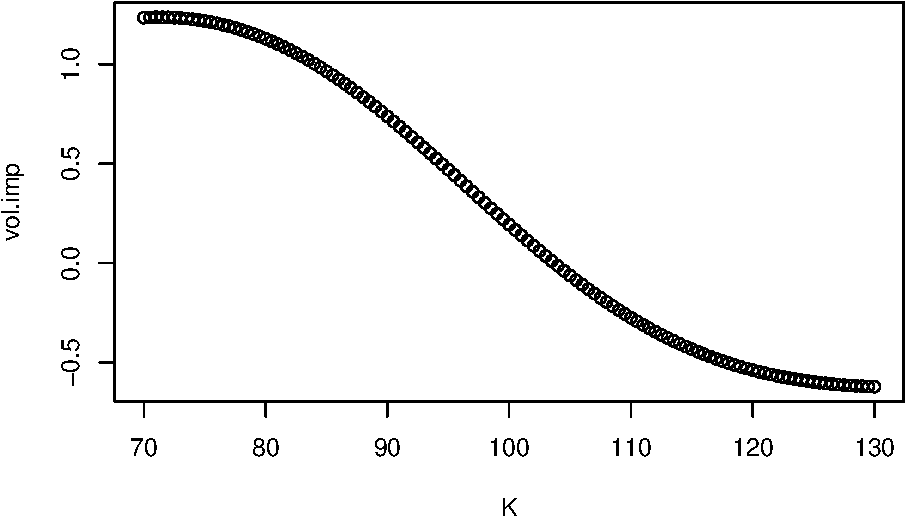
\includegraphics{TP-VannaVolga_files/figure-latex/unnamed-chunk-10-1.pdf}

\hypertarget{pricing-a-digital-call}{%
\section{Pricing a digital call}\label{pricing-a-digital-call}}

Recall that a digital call with strike \(K\) pays one euro if
\(S_T \geq K\), and nothing otherwise.

Using the same logic as in the previous question, price a digital call,
maturity \(T=1\), struck at \(K=105\).

\begin{Shaded}
\begin{Highlighting}[]
\NormalTok{r}\OtherTok{\textless{}{-}}\DecValTok{0}
\NormalTok{b}\OtherTok{\textless{}{-}}\DecValTok{0}
\NormalTok{T}\OtherTok{\textless{}{-}}\DecValTok{1}
\NormalTok{Spot }\OtherTok{\textless{}{-}} \DecValTok{100}
\NormalTok{K }\OtherTok{\textless{}{-}} \DecValTok{105}

\NormalTok{epsi }\OtherTok{\textless{}{-}} \FloatTok{0.0001}


\NormalTok{VolData.ATM }\OtherTok{\textless{}{-}}\NormalTok{ VolData[[}\DecValTok{2}\NormalTok{]][}\DecValTok{2}\NormalTok{]}

\NormalTok{f }\OtherTok{\textless{}{-}} \ControlFlowTok{function}\NormalTok{(}\AttributeTok{vol=}\NormalTok{VolData.ATM, }\AttributeTok{spot=}\NormalTok{Spot)\{}
  \FunctionTok{GBSPrice}\NormalTok{(}\AttributeTok{PutCall=}\StringTok{\textquotesingle{}c\textquotesingle{}}\NormalTok{, }\AttributeTok{S=}\NormalTok{spot, }\AttributeTok{K=}\NormalTok{K}\SpecialCharTok{{-}}\NormalTok{epsi, }\AttributeTok{T=}\NormalTok{T, }\AttributeTok{r=}\NormalTok{r, }\AttributeTok{b=}\NormalTok{b, }\AttributeTok{sigma=}\NormalTok{vol)}
\NormalTok{\}}
\NormalTok{B.vega }\OtherTok{\textless{}{-}} \FunctionTok{Vega}\NormalTok{(f, VolData.ATM, Spot)}
\NormalTok{B.vanna }\OtherTok{\textless{}{-}} \FunctionTok{Vanna}\NormalTok{(f, VolData.ATM, Spot)}
\NormalTok{B.volga }\OtherTok{\textless{}{-}} \FunctionTok{Volga}\NormalTok{(f, VolData.ATM, Spot)}
\FunctionTok{print}\NormalTok{(}\StringTok{"vega for K=105 {-} espilon"}\NormalTok{)}
\end{Highlighting}
\end{Shaded}

\begin{verbatim}
## [1] "vega for K=105 - espilon"
\end{verbatim}

\begin{Shaded}
\begin{Highlighting}[]
\NormalTok{B.vega}
\end{Highlighting}
\end{Shaded}

\begin{verbatim}
## [1] 11.96731
\end{verbatim}

\begin{Shaded}
\begin{Highlighting}[]
\FunctionTok{print}\NormalTok{(}\StringTok{"vanna for K=105 {-} espilon"}\NormalTok{)}
\end{Highlighting}
\end{Shaded}

\begin{verbatim}
## [1] "vanna for K=105 - espilon"
\end{verbatim}

\begin{Shaded}
\begin{Highlighting}[]
\NormalTok{B.vanna}
\end{Highlighting}
\end{Shaded}

\begin{verbatim}
## [1] 12.47117
\end{verbatim}

\begin{Shaded}
\begin{Highlighting}[]
\FunctionTok{print}\NormalTok{(}\StringTok{"volga for K=105 {-} espilon"}\NormalTok{)}
\end{Highlighting}
\end{Shaded}

\begin{verbatim}
## [1] "volga for K=105 - espilon"
\end{verbatim}

\begin{Shaded}
\begin{Highlighting}[]
\NormalTok{B.volga}
\end{Highlighting}
\end{Shaded}

\begin{verbatim}
## [1] 0.04725749
\end{verbatim}

\begin{Shaded}
\begin{Highlighting}[]
\NormalTok{b.risk.moins }\OtherTok{\textless{}{-}} \FunctionTok{c}\NormalTok{(B.vega, B.vanna, B.volga)}
\NormalTok{X.moins }\OtherTok{\textless{}{-}} \FunctionTok{solve}\NormalTok{(A, b.risk.moins)}

\NormalTok{O.BS.moins }\OtherTok{\textless{}{-}} \FunctionTok{GBSPrice}\NormalTok{(}\AttributeTok{PutCall=}\StringTok{\textquotesingle{}c\textquotesingle{}}\NormalTok{, }\AttributeTok{S=}\DecValTok{100}\NormalTok{, }\AttributeTok{K=}\NormalTok{K}\SpecialCharTok{{-}}\NormalTok{epsi, }\AttributeTok{T=}\NormalTok{T, }\AttributeTok{r=}\NormalTok{r, }\AttributeTok{b=}\NormalTok{b, }\AttributeTok{sigma=}\NormalTok{VolData[[}\DecValTok{2}\NormalTok{]][}\DecValTok{2}\NormalTok{])}


\NormalTok{somme }\OtherTok{\textless{}{-}} \DecValTok{0}
\ControlFlowTok{for}\NormalTok{ (i }\ControlFlowTok{in} \DecValTok{1}\SpecialCharTok{:}\DecValTok{3}\NormalTok{) \{}
\NormalTok{  somme }\OtherTok{\textless{}{-}}\NormalTok{ somme }\SpecialCharTok{+}\NormalTok{ X.moins[i]}\SpecialCharTok{*}\NormalTok{(C.M[i]}\SpecialCharTok{{-}}\NormalTok{C.BS[i])}
\NormalTok{\}}
\NormalTok{O.M.moins }\OtherTok{\textless{}{-}}\NormalTok{ O.BS.moins }\SpecialCharTok{+}\NormalTok{ somme}

\FunctionTok{print}\NormalTok{(}\StringTok{"price with BS for K=105 {-} espilon"}\NormalTok{)}
\end{Highlighting}
\end{Shaded}

\begin{verbatim}
## [1] "price with BS for K=105 - espilon"
\end{verbatim}

\begin{Shaded}
\begin{Highlighting}[]
\FunctionTok{print}\NormalTok{(O.BS.moins)}
\end{Highlighting}
\end{Shaded}

\begin{verbatim}
## [1] 9.881693
\end{verbatim}

\begin{Shaded}
\begin{Highlighting}[]
\FunctionTok{print}\NormalTok{(}\StringTok{"price ajusted for K=105 {-} espilon"}\NormalTok{)}
\end{Highlighting}
\end{Shaded}

\begin{verbatim}
## [1] "price ajusted for K=105 - espilon"
\end{verbatim}

\begin{Shaded}
\begin{Highlighting}[]
\FunctionTok{print}\NormalTok{(O.M.moins)}
\end{Highlighting}
\end{Shaded}

\begin{verbatim}
## [1] 9.881693
\end{verbatim}

\begin{verbatim}
## [1] "vega for K=105 - espilon"
\end{verbatim}

\begin{verbatim}
## [1] 11.96731
\end{verbatim}

\begin{verbatim}
## [1] "vanna for K=105 - espilon"
\end{verbatim}

\begin{verbatim}
## [1] 12.47142
\end{verbatim}

\begin{verbatim}
## [1] "volga for K=105 - espilon"
\end{verbatim}

\begin{verbatim}
## [1] 0.04727951
\end{verbatim}

\begin{verbatim}
## [1] "price with BS for K=105 + espilon"
\end{verbatim}

\begin{verbatim}
## [1] 9.881618
\end{verbatim}

\begin{verbatim}
## [1] "price ajusted for K=105 + espilon"
\end{verbatim}

\begin{verbatim}
## [1] 9.881618
\end{verbatim}

\begin{verbatim}
## [1] "price for a digital call paying 2*epsi"
\end{verbatim}

\begin{verbatim}
## [1] 7.545588e-05
\end{verbatim}

\begin{verbatim}
## [1] "price for a digital call paying 1"
\end{verbatim}

\begin{verbatim}
## [1] 0.3772794
\end{verbatim}

\end{document}
